\uuid{INtA}
\exo7id{5525}
\auteur{rouget}
\organisation{exo7}
\datecreate{2010-07-15}
\isIndication{false}
\isCorrection{true}
\chapitre{Courbes planes}
\sousChapitre{Courbes paramétrées}

\contenu{
\texte{
La courbe orthoptique d'une courbe $(\mathcal{C})$ est le lieu  des points du plan d'où l'on peut mener (au moins) deux
tangentes à $(\mathcal{C})$, orthogonales. Déterminer l'orthoptique de $(\mathcal{C})$ dans chacun des cas suivants~:
}
\begin{enumerate}
    \item \question{$(\mathcal{C})$ est un astroïde de paramétrisation $\left\{\begin{array}{l}
x=a\cos^3t\\
y=a\sin^3t
\end{array}\right.$, $a>0$ donné.}
    \item \question{$(\mathcal{C})$ est l'arc paramétré~:~$\left\{
\begin{array}{l}
x=t^2-2t\\
y=2t^3-3t^2
\end{array}
\right.$.}
    \item \question{$(\mathcal{C})$ est l'ellipse d'équation $\frac{x^2}{a^2}+\frac{y^2}{b^2}=1$, $(a,b)\in]0,+\infty[^2$.}
\reponse{
On a vu dans l'exercice \ref{exo:routhe1}, que la tangente $(T_t)$ en $M(t)$ est toujours dirigée par le vecteur $\vec{u}(t)=(-\cos t,\sin t)$. Une équation de la tangente en $M(t)$ est donc $\sin t(x-a\cos^3t)+\cos t(y-a\sin^3t)=0$ ou encore

$$x\sin t+y\cos t=a\sin t\cos t\;(T_t).$$

Soit $(t,u)\in[-\pi,\pi]^2$. 

$$(T_t)\bot(T_u)\Leftrightarrow\vec{u}(t)|\vec{u}(u)=0\Leftrightarrow\cos t\cos u+\sin t\sin u=0\Leftrightarrow\cos(t-u)=0\Leftrightarrow u\in t+\frac{\pi}{2}+\pi\Zz.$$

Il est alors clair que l'orthoptique est l'ensemble des points d'intersection des tangente $(T_t)$ et $(T_{t+\frac{\pi}{2}})$ quand $t$ décrit $\Rr$.

\begin{align*}\ensuremath
M(x,y)\;(T_t)\cap(T_{t+\frac{\pi}{2}})&\Leftrightarrow
\left\{
\begin{array}{l}
x\sin t+y\cos t=a\sin t\cos t\\
x\cos t-y\sin t=-a\sin t\cos t
\end{array}
\right.
\\
 &\Leftrightarrow
x=-\left|
\begin{array}{cc}
a\sin t\cos t&\cos t\\
-a\sin t\cos t&-\sin t
\end{array}
\right|
\;\mbox{et}
\;
y=-\left|
\begin{array}{cc}
\sin t&a\sin t\cos t\\
\cos t&-a\sin t\cos t
\end{array}
\right|
\\
 &\Leftrightarrow x=a\sin t\cos t(-\cos t+\sin t)\;\mbox{et}\;y=a\sin t\cos t(\cos t+\sin t)
\end{align*}

L'orthoptique cherchée est la courbe $t\mapsto\left(
\begin{array}{c}
a\sin t\cos t(-\cos t+\sin t)\\
a\sin t\cos t(\cos t+\sin t)
\end{array}
\right)$.

$$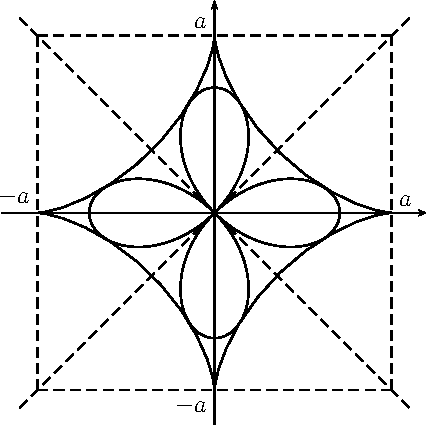
\includegraphics{../images/img005525-1}$$
}
\end{enumerate}
}
